\subsection{Differentiation}

\subsubsection{Tangent Lines}
We are often interested in rates of change. We know the rate of change of a linear function to be its slope which is a constant. However, for nonlinear functions, the rate of change is not constant. We can determine the instantaneous rate of change of a function at a point $P$ by drawing a line tangent to the curve at that point. This line is not always easy to find so we start by drawing a secant line that intersects the curve at two points, $P$ and $Q$.\\
\centerline{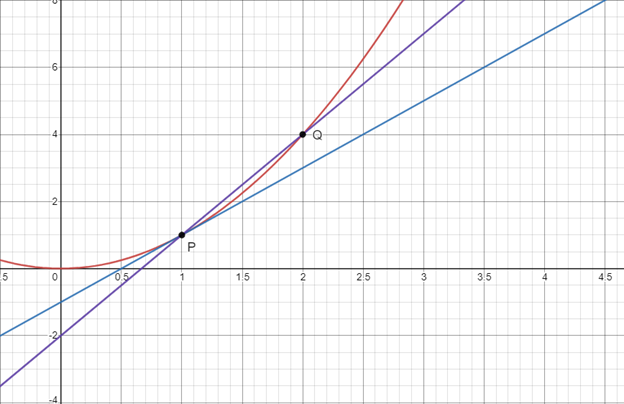
\includegraphics[scale =0.7]{Images/DifferentialCalculusPictures/Tangent.png}}
To find the tangent line, we can take the limit as the point $Q$ on the secant line approaches the point $P$.\\
The slope of the secant line is $m_{sec}=\dfrac{f(x_Q)-f(x_P)}{x_Q-x_P}$\\
We can define $x_Q=x_P+h$ where $h$ is the distance between the points so,\\ ${m_{sec}=\dfrac{f(x_P+h)-f(x_P)}{x_P+h-x_P}=\dfrac{f(x_P+h)-f(x_P)}{h}}$\\
Because we are interested in the case where $x_P=x_Q$, we take the limit as $h\to 0$:\\
$m_{tan}=\displaystyle{\lim \limits_{h\to 0}\dfrac{f(x_P+h)-f(x_P)}{h}}$\\
This is in fact the definition of the derivative. Put simply, the derivative measures rates of change between two variables. It is denoted by $f'(x)$ or $\frac{dy}{dx}$.\\
$$f'(x)=\lim\limits_{h\to 0}\frac{f(x+h)-f(x)}{h}=\lim_{x\to a}\frac{f(x)-f(a)}{x-a}$$
So, the tangent line at a point $a$ can be defined as $$y=f'(a)x+f(a)$$
Ex: Find the line tangent to $x^3$ at $(2,8)$
\begin{align*}
    &f'(2)=\lim\limits_{h\to 0}\frac{(2+h)^3-2^3}{h}=\lim\limits_{h\to 0}\frac{8+12h+6h^2+h^3-8}{h}=\lim\limits_{h\to 0}(12+6h+h^2)=12\\
    &y=f'(2)x+f(2)=12x+8
\end{align*}
It is important to note that a function must be continuous in order for it to be differentiable.

\subsubsection{Derivative Laws}
We can derive various derivative laws that will make calculating derivatives far easier. They stem from these derivations:\\
Derivative of a Constant:
\begin{align*}
    \frac{d}{dx}c&=\lim_{h\to 0}\frac{c-c}{h}\\
    \frac{d}{dx}c&=0
\end{align*}
Derivative of a Polynomial:
\begin{align*}
    \frac{d}{dx}x^n&=\lim\limits_{h\to 0}\frac{(x+h)^n-x^n}{h}\text{ for $n$ is a constant}\\
    \text{Binomial theorem: }& (a+b)^n=\prescript{}{n}{C}_0a^n+\prescript{}{n}{C}_1a^{n-1}b+\prescript{}{n}{C}_2a^{n-2}b^2+\cdots+\prescript{}{n}{C}_{n-1}ab^{n-1}+\prescript{}{n}{C}_nb^n\\
    \frac{d}{dx}x^n&=\lim\limits_{h\to 0}\frac{x^n+nx^{n-1}h+\cdots+nh^{n-1}+h^n-x^n}{h}\\
    \frac{d}{dx}x^n&=\lim\limits_{h\to 0}(nx^{n-1}+n(n-1)x^{x-2}h+\cdots+h^{n-1})\\
    \frac{d}{dx}x^n&=nx^{n-1}
\end{align*}
Ex: $\frac{d}{dx}(6x^5)=30x^4$\\
Note that coefficients do not change the value of the derivative. I did not prove this but it's easy to see.\\
Ex2: $\frac{d}{dx}\sqrt{x}=\frac{1}{2}x^{-\frac{1}{2}}=\frac{1}{2\sqrt{x}}$\\
We can define the multiplication of two functions with the product rule:
\begin{align*}
    \frac{d}{dx}(f(x)g(x))&=\lim_{h\to 0}\frac{f(x+h)g(x+h)-f(x)g(x)}{h}\\
    &=\lim_{h\to 0}\frac{f(x+h)g(x+h)-f(x)g(x)-f(x)g(x+h)+f(x)g(x+h)}{h}\\
    &=\lim_{h\to 0}\left(f(x)\frac{g(x+h)-g(x)}{h}+g(x+h)\frac{f(x+h)-f(x)}{h}\right)\\
    &=f(x)g'(x)+g(x)f'(x)
\end{align*}
Product Rule with 3 Functions:
\begin{align*}
    (uvw)'=u'vw+v'uw+w'uv
\end{align*}
Quotient Rule:
\begin{align*}
    \frac{d}{dx}\left(\frac{f(x)}{g(x)}\right)&=\lim_{h\to 0}\frac{\frac{f(x+h)}{g(x+h)}-\frac{f(x)}{g(x)}}{h}\\
    &=\lim_{h\to 0}\frac{g(x)f(x+h)-f(x)g(x+h)}{hg(x)g(x+h)}\\
    &=\lim_{h\to 0}\frac{g(x)f(x+h)-f(x)g(x+h)+g(x+h)f(x+h)-g(x+h)f(x+h)}{hg(x)g(x+h)}\\
    &=\lim_{h\to 0}\frac{g(x+h)\frac{f(x+h)-f(x)}{h}-f(x+h)\frac{g(x+h)-g(x)}{h}}{g(x)g(x+h)}\\
    &=\frac{g(x)f'(x)-f(x)g'(x)}{(g(x))^2}
\end{align*}
Reciprocal Rule:
\begin{align*}
    \frac{d}{dx}\brround{\frac{1}{v}}=-\frac{v'}{v^2}
\end{align*}
Ex: $\dfrac{d}{dx}x^2\cos x=2x\cos x-x^2\sin x$\\
By extension of the quotient rule, we can also define the derivative of a reciprocal to be
$$\frac{d}{dx}\frac{1}{x}=\frac{-1}{x^2}$$
Higher Order Derivatives:\\
This is taking the derivative of a derivative, generally expressed as $$\frac{d}{dx}\brround{\frac{dy}{dx}}=\frac{d^2y}{dx^2}=f''(x)$$
Ex: find $f''(x)$ for $f(x)=x^3-x$
\begin{align*}
    &f'(x)=3x^2-1\\
    &f''(x)=6x
\end{align*}
\begin{align*}
    \text{Ex2: }&\frac{d^n}{dx^n}x^n\\
    &\frac{d}{dx}x^n=nx^{n-1}\\
    &\frac{d^2}{dx^2}x^n=n(n-1)x^{n-2}\\
    &\frac{d^3}{dx^3}x^n=n(n-1)(n-2)x^{n-3}\\
    &\frac{d^{n-1}}{dx^{n-1}}x^n=n(n-1)(n-2)\cdots(3)(2)x^1\\
    &\therefore\frac{d^n}{dx^n}x^n=n!
\end{align*}

\subsubsection{Derivatives of Trigonometric Functions}
Derivative of $\sin x$:
\begin{align*}
    \frac{d}{dx}\sin (x)&=\lim_{h\to 0}\frac{\sin(x+h)-\sin (x)}{h}\\
    &=\lim_{h\to 0}\frac{\sin(x)\cos(h)+\sin(h)\cos(x)-\sin(x)}{h}\\
    &=\sin(x)\lim_{h\to 0}\left(\frac{\cos(h)-1}{h}\right)+\cos(x)\lim_{h\to 0}\left(\frac{sin(h)}{h}\right)\\
    &=\cos(x)
\end{align*}
Derivative of $\cos x$:
\begin{align*}
    \frac{d}{dx}\cos(x)&=\lim_{h\to 0}\frac{\cos(x+h)-\cos(x)}{h}\\
    &=\lim_{h\to 0}\frac{\cos(x)\cos(h)-\sin(x)\sin(h)-\cos(x)}{h}\\
    &=\cos(x)\lim_{h\to 0}\left(\frac{\cos(h)-1}{h}\right)-\sin(x)\lim_{h\to 0}\left(\frac{sin(h)}{h}\right)\\
    &=-\sin(x)
\end{align*}
Derivative of $\tan x$:\\
$\dfrac{d}{dx}\tan x=\dfrac{d}{dx}\dfrac{\sin x}{\cos x}=\dfrac{\cos x\cos x+\sin x\sin x}{\cos^2x}=\dfrac{1}{\cos^2x}=\sec^2x$\\
\\
Derivative of $\csc x$:\\
$\dfrac{d}{dx}\dfrac{1}{\sin x}=-\dfrac{\cos x}{\sin^2 x}=-\csc x\cot x$\\
\\
List of Trig Derivatives:\\
\begin{align*}
    &\frac{d}{dx}\sin x=\cos x &\frac{d}{dx}\csc x = -\csc x\cot x\\
    &\frac{d}{dx}\cos x=-\sin x &\frac{d}{dx}\sec x=\sec x\tan x\\
    &\frac{d}{dx}\tan x =\sec^2 x &\frac{d}{dx}\cot x=-\csc^2 x
\end{align*}

\subsubsection{The Chain Rule}
$$\frac{dy}{dx}=\frac{dy}{du}\frac{du}{dx}$$ or also $$\frac{d}{dx}f(g(x))=f'(g(x))g'(x)$$
This gives us the tools we need to differentiate more complicated functions.
Ex: $\frac{d}{dx}(x^2+5x)^3=(x^2+5x)^3(2x+5)$\\
Ex2: $\frac{d}{dx}\cos(x^2)=-2x\sin(x^2)$\\
Ex3: Find values for $a$ and $b$ such that $f(x)$ is differentiable everywhere:
\begin{align*}
    &f(x)=\left\{\begin{matrix}
    x^3+ax+b,\,x\leq 0\\
    x+x^3\sin\brround{\frac{1}{x}}
    ,\,x>0\end{matrix}\right.\\
    &\text{check that $f(x)$ is continuous at $x=0$}\\
    &\lim_{x\to0^-}f(x)=\lim_{x\to0^+}=f(0)\Ra\lim_{x\to 0^+}\brround{x+x^3\sin\brround{\frac{1}{x}}}=b=0\\
    &\text{chech that $f'(x)$ is continuous at $x=0$}\\
    &\lim_{h\to 0}\frac{f(0+h)-f(0)}{h}\text{ must exist}\\
    &\text{recall }\lim_{x\to 0^-}f(x)=\lim_{x\to0^+}f(x)=f(0)=0\\
    &\therefore \lim_{h\to 0}\frac{f(0+h)-f(0)}{h}=\lim_{h\to0}\frac{f(h)}{h}\\
    &\lim_{h\to 0^-}\frac{h^3+ah}{h}=\lim_{h\to 0^+}\frac{h+h^3\sin\brround{\frac{1}{h}}}{h}\\
    &\lim_{h\to0^-}(h^2+a)=\lim_{h\to0^+}\brround{1+h^2\sin\brround{\frac{1}{h}}}\\
    &a=1\\
    &\to a=1,\,b=0
\end{align*}